\chapter{評価実験}
提案手法の有効性を示すため2種類の実験を行った.いずれもタスクの対象としてconnect4を扱っている.\\
1つ目の実験(以下データ実験と表記)はコンピュータ同士の対戦データを用いて提案手法による想定図の妥当性を評価した.\\
2つ目の実験(以下インタフェース実験と表記)は自作のGUIシステムを用いた提案手法の学習支援ツールとしての有効性を評価した.
本章ではデータ実験,インタフェース実験の詳細と結果を記載する.



\section{データ実験}
\label{chap:evaluation}
提案手法と後に述べる比較手法によるゲーム結果(後で勝敗も含める)の予測精度を比較した.
\subsection{データセット}
alphazero\_baselinモデル同士の対戦データ2000局分(盤面数:61049)を使用した.いずれもいずれも弱いAIが先番のデータを使用している.これは弱いAIが後番の場合評価関数の変動が極めて小さくなることと,弱い側が先番を選択することが指導において一般的とされるためである.



\subsection{データ実験の評価指標}
提案手法と次節で述べる比較手法による予測の精度を独自に定義した2つの定義group prediction rate($P_g$),stone prediction rate($P_s$)によって計測した.stone prediction rate, group prediction rateの詳細な定義は付録Aに記載する.
それぞれが,最終盤面において4つ以上連続して並ぶ石と組み合わせ(以下fatal stone,fatal groupと記載)の座標に対する予測精度を表している.

本論文が提案する提案指標(group prediction rate, stone prediction rate)の計算において,盤面の座標は図\ref{fig:index}のように定められる.
\begin{figure}[t]
	\centering
	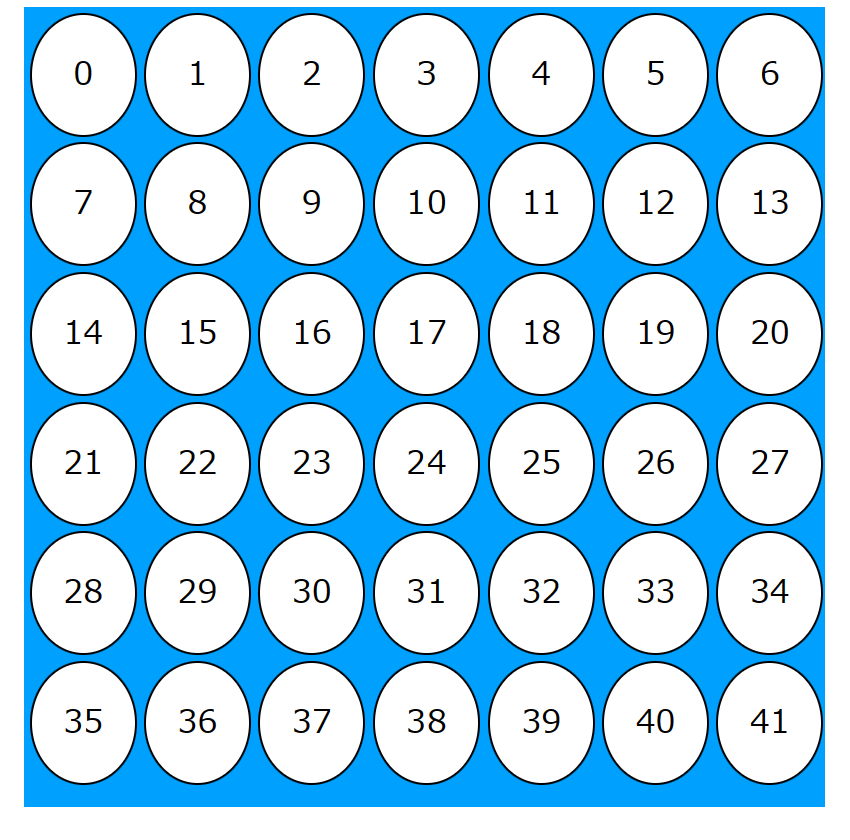
\includegraphics[width=300pt]{./figure/index.png}
	\caption{盤面の座標番号}
	\label{fig:index}
\end{figure}
図\ref{fig:fatalGroup}のようにゲームの終了状態において,4つ以上連続してつながっている石の座標$F_s$(fatal stoneの集合)とその組み合わせ$F_g$(fatal groupの集合)を記録する.
図\ref{fig:fatalGroup}の盤面は$\{17, 18, 19, 20, 24, 31, 38\}$の7つのfatal stoneと$\{[17, 18, 19, 20], [17, 24, 31, 38]\}$の2つのfatal groupを持つ.
\begin{figure}[t]
	\centering
	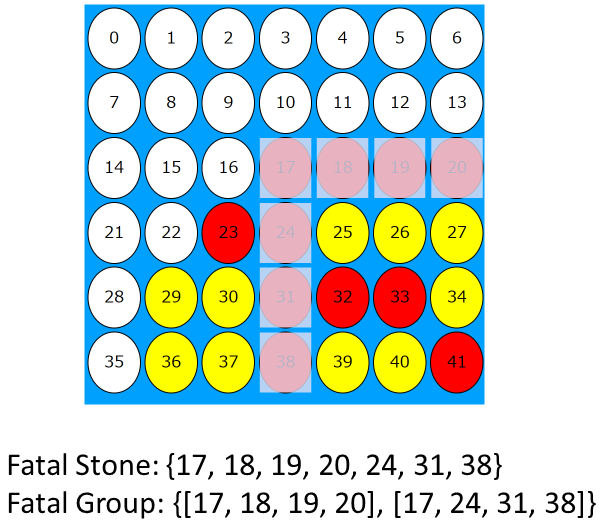
\includegraphics[width=\linewidth]{./figure/fatalGroup.png}
	\caption{fatalStoneとfatalGroup}
	\label{fig:fatalGroup}
\end{figure}
group prediction rate($P_g$), stone prediction rate($P_s$)は実際のゲームにおけるfatal groupとfatal stoneの集合(それぞれ$R_s, R_g$とする)とAIの予測によるfatal stoneとfatal groupの集合($F_g, F_s$)を比較する指標である.
どちらも値が高ければ高い程予測の精度が高いことを表す.


\subsection{group prediction rate}
group prediction rate はfatal groupの予測精度を示す2値(0または1)の指標である.
\begin{equation}
	{P_g = 1 \quad \textrm{If} \quad F_g \cap R_g \ne \phi \quad \textrm{Else} \quad 0}
\end{equation}
例外として$R_g=\phi$(引き分け)の場合,$F_g$も空集合であるならばgroup prediction rateは1となる.
\subsection{stone prediction rate}
stone prediction rateはfatal stoneの予測精度を示す.stone prediction rateの値域は[0, 1]である.
(Count()は集合の要素数を数える関数)
\begin{equation}
	{P_s = \textrm{Min}(\frac{\textrm{Count}(F_s \cap R_s)}{4}, 1)  }
\end{equation}
例外として$R_s=\phi$(引き分け)の場合,$F_s$も空集合であるならばstone prediction rateは1となる.


例えば,実際の結果と予測結果が図\ref{fig:cal-compare}の様になる場合, $R_g$と$F_g$は$[17, 24, 31, 38]$が共通しているためgroup prediction rateは1, stone prediction rateは$\frac{4}{4}=1$となる.
\begin{figure}[t]
	\centering
	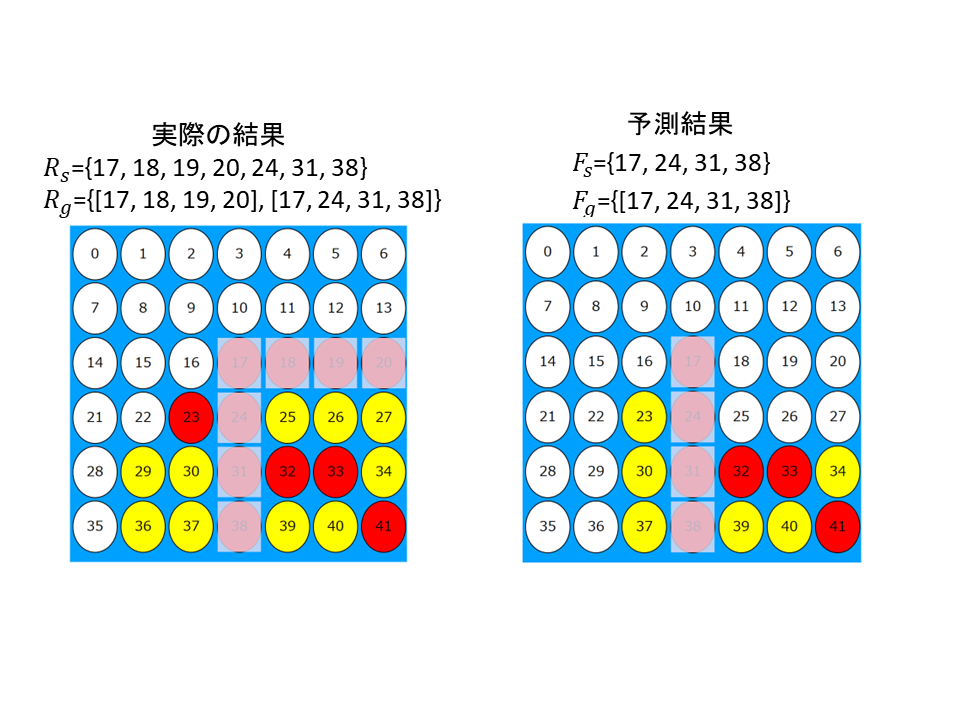
\includegraphics[width=\linewidth]{./figure/cal-compare.png}
	\caption{予測結果の例}
	\label{fig:cal-compare}
\end{figure}


\subsection{比較手法}
提案手法と比較手法はそれぞれ以下の方式で予測を行う.
比較手法の詳細なアルゴリズムは付録\ref{chap:alg}に記載した.
\newpage
\begin{itemize}
	\item 比較手法: 探索の開始地点から最も訪問回数が大きい選択肢を選び続けたたどり着いた最終局面の$F_s, F_g$を用いる.
	\item 提案手法: 集めた盤面における4つ繋がっている石を集計し,最も出現頻度が高いfatal group を$F_s$, 2番目までに出現頻度が高いfatal groupを$F_g$として用いる.組み合わせを2つ記録する理由は下の図のように最終的に繋がっている組み合わせが2つある可能性を考慮するためである.
\end{itemize}
図\ref{fig:compare}は比較手法と提案手法の概要を示している.
\begin{figure}[t]
	\centering
	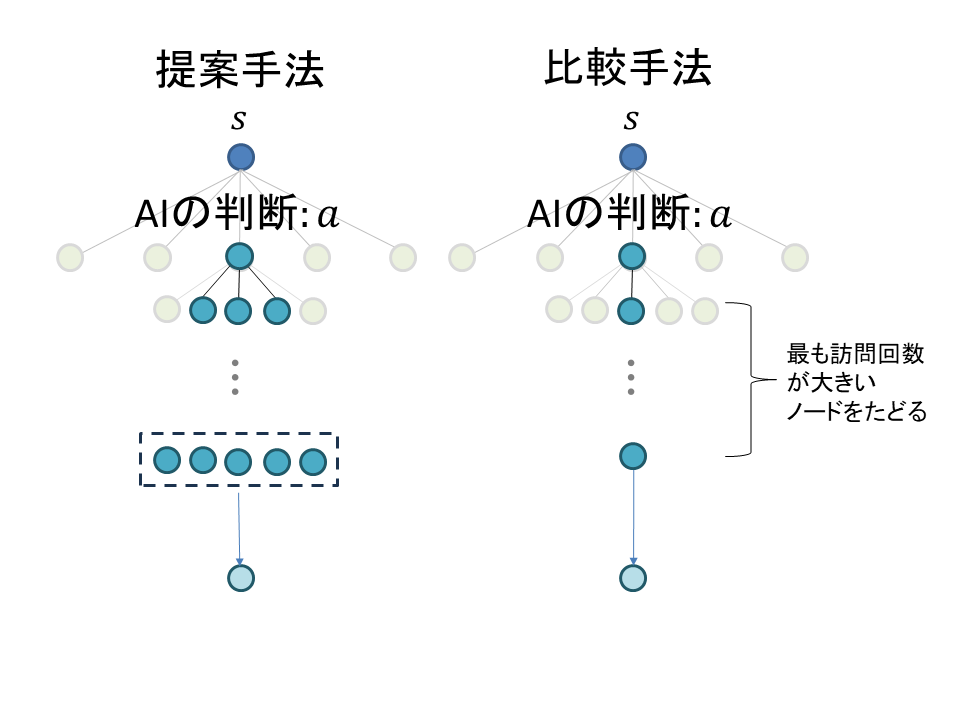
\includegraphics[width=\linewidth]{./figure/compare-image.png}
	\caption{提案手法と比較手法の比較}
	\label{fig:compare}
\end{figure}
また,提案手法による予測が図\ref{fig:g-example}のようになる場合,$[1,2,3,4]$が最も多く含まれているfatal group
であり,2番目は$[1, 9, 17, 25]$である.そのため,提案手法全体による予測結果は$F_g=\{[1, 2, 3, 4], [1, 9, 17, 25]\}, F_s=\{1, 9, 17, 25\}$となる.
\begin{figure}[t]
	\centering
	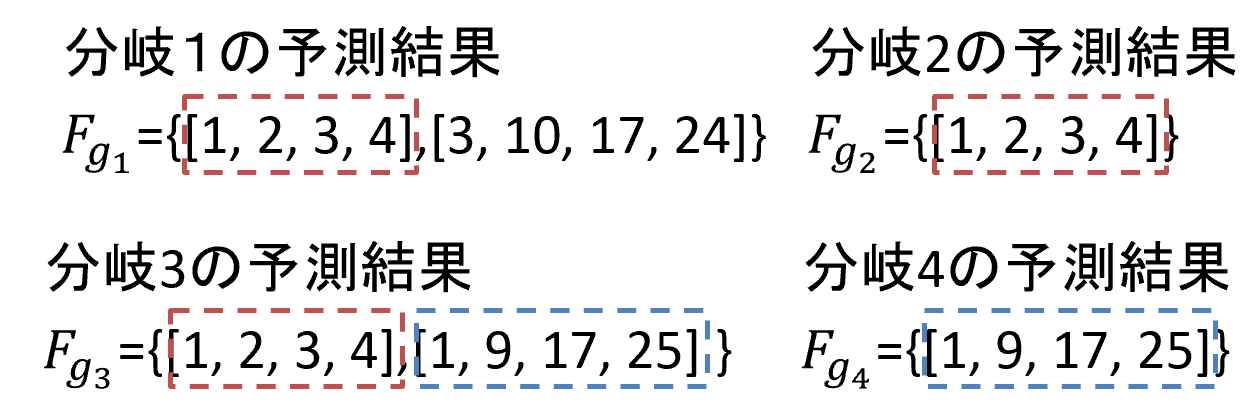
\includegraphics[width=\linewidth]{./figure/g-example.png}
	\caption{提案手法による予測}
	\label{fig:g-example}
\end{figure}

\subsection{データ実験における提案指標の計測}

\begin{enumerate}
	\item 比較手法: 決定木の走査によりたどり着いた$F_s, F_g$によってstone prediction rate, group prediction rateを計算した
	\item 提案手法: 第3章で述べたアルゴリズムによって収集された最終状態の集合$S=\{s_{edge_1}, s_{edge_2}, ..., s_{edge_{k^l}}\}$
	    を指標ごとにグループ化する.
		\begin{itemize}
			\item group prediction rate: fatal groupによって$S$をグループ化してできた集合$\{S_{g_1}, S_{g_2}, ..., S_{g_n}\}$($S_{g_i}$は組み合わせ$g_i$がfatal groupとなっている盤面の集合)
			を要素が多い順に2つ取り出す.抽出された2つの集合$\{S_{g_{m_1}}, S_{g_{m_2}}\}$における$\{g_{m_1}, g_{m_2}\}$で構成される集合を$F_g$とし,group prediction rateを計算した.
			\item stone prediction rate: $g_{m_1}$を$F_s$とし,stone prediction rateを計算した.
		\end{itemize}
		
\end{enumerate}

\subsection{実験結果(データ実験)}
盤面データのうち,手数(盤面上の赤または黄色)が13$\sim$24のものに対して実験を行った.
表\ref{table:result-online}に実験結果(group prediction rate,stone prediction rateの平均値)を示す.いずれの場合もgroup prediction rateにおいて提案手法は比較手法より高い値を示した.
表中に記載した「補間」の詳細は付録\ref{chap:alg}に記載する.
\begin{table}[H]
	\caption{実験結果:最終状態の予測}
	\centering
	\scalebox{0.98}[0.98]{
		\begin{tabular}{c|c|c|c|c}
			\multicolumn{1}{c}{} & \multicolumn{2}{|c|}{mean group prediction rate} 
			& \multicolumn{2}{c|}{mean stone prediction rate}\\ \hline \hline
			手数(盤面数, 補間の有無)  & 比較手法  & 提案手法 & 比較手法 & 提案手法  \\ \hline
			19-24(9862, 無)  & 0.43  & \bf{0.60} & \bf{0.62}  & 0.55  \\
			19-24(9862, 有) & 0.44   & \bf{0.63} & \bf{0.63}  & 0.61   \\
			13-24(21022, 無) & 0.37  & \bf{0.52} & \bf{0.56} & 0.55   \\
			13-24(21022, 有)   & 0.37 & \bf{0.55} & \bf{0.56} & 0.55   \\
		\end{tabular}
	}
	\label{table:result-online}
\end{table}
\subsection{考察(データ実験)}
提案手法はgroup prediction rateにおいて比較手法より高い結果を示した.
この結果は提案手法がfatal groupを予測する能力に長けている事を意味する.
比較手法によって予測されるfatal groupの集合は
最も訪問回数が大きい軌跡が辿り着く1つの最終状態のものである.
一方で提案手法により予測されるfatal groupの集合は,複数の軌跡がそれぞれに辿り着く最終状態のfatal groupの多数派投票によって決定され,第1位と第2位のものが採用される.\\
使用した対戦データは対戦者間の強さに差があり,予測は強い側の決定木を用いている.
決定木内での最も訪問回数の大きい軌跡(以下主軌跡と記載)はAIが予測する双方が最善を尽くした場合の進行と解釈される.
実際に弱いAIと対戦を行う際には,弱いAIは強いAIが最善とみなす行動(最も訪問回数が大きい行動)を必ずしも選択しない.
そのため,実際の進行は,比較手法に用いられる主軌跡とは異なる可能性が高い.
提案手法では,主軌跡を含む複数の軌跡を用いているため,より精度の高い予測が可能になったと考えられる.\\
また,提案手法は2組のfatal groupを保存することから比較手法よりも予測するfatal groupの数が多くなる傾向にあるため,必然的にgroup prediction rateの値も大きくなったとも考えられる.


\section{インタフェース実験}
提案手法の人間に対する有効性を示すため以下のように自作したconnect4の学習支援システムを用いて実験を行った.
自作システムの開始画面は\ref{fig:basic}のように構成されており,右側の青い正方形の部分をクリックすることでconnect4をプレイできる.
実験対象者は大学生,大学院生の22名(男性17名:女性5名)となった.
\begin{figure}[t]
    \centering
    \setlength{\fboxsep}{1pt} % フレームの余白を調整
    \setlength{\fboxrule}{1pt} % フレームの太さを調整
    \fbox{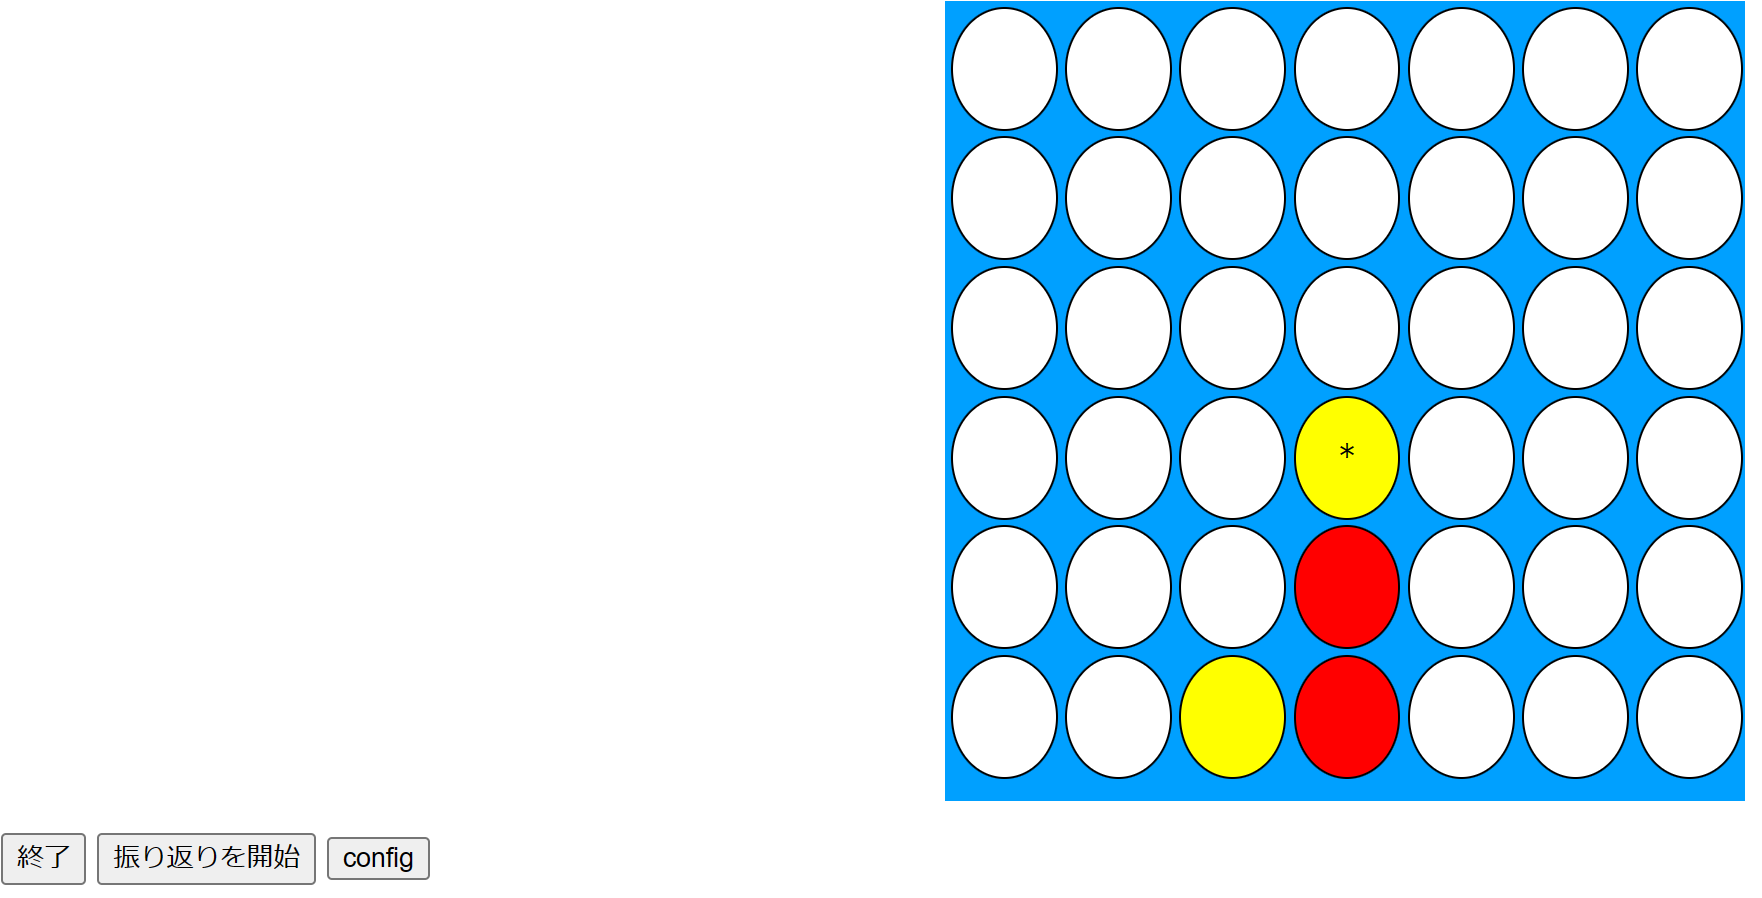
\includegraphics[width=\linewidth]{./figure/basicSystem.png}}
    \caption{開始画面}
    \label{fig:basic}
\end{figure}

\subsection{実験手順}
実験は被験者1人あたりにつき3回行われ,1回目と2回目を第1段階(提案手法による学習),3回目を第2段階(被験者同士の対戦)とした.
ここでは第1段階である提案手法の学習について述べる.
\newpage
\paragraph{第1段階(提案手法による学習)}~
\par 提案システムを用いた学習はさらに
\begin{itemize}
	\item AIシステム(alphazero\_baseline)との対戦
	\item 提案手法によるゲームの振り返り
\end{itemize}
の2ステップに分けられる.
まず,図\ref{fig:basic}の画面をクリックしながらAIとの対戦を行う.実験ではユーザーを先番(赤)とした.


AIシステムとの対戦が終了するとシステムは「振り返りモード」に移行する.
「振り返りモード」は図\ref{fig:lookBack}のように構成される.
右側に直前のゲームの振り返りたい地点の盤面が表示され,ユーザーは数字の描かれたボタンを押すことで
AIによる進行図を閲覧できる.進行図は提案手法または比較手法によって生成される.
インタフェースの詳しい構成は付録\ref{chap:system}に記載した.
また,「振り返りモード」は第3章で定義した重要度$I(s)$が最も高い地点から開始する.

実験の際には被験者をグループA(提案手法による進行図を見せるグループ)とグループB(比較手法による進行図を見せるグループ)に分類した.
\begin{figure}[t]
	\centering
    \setlength{\fboxsep}{1pt} % フレームの余白を調整
    \setlength{\fboxrule}{1pt} % フレームの太さを調整
    \fbox{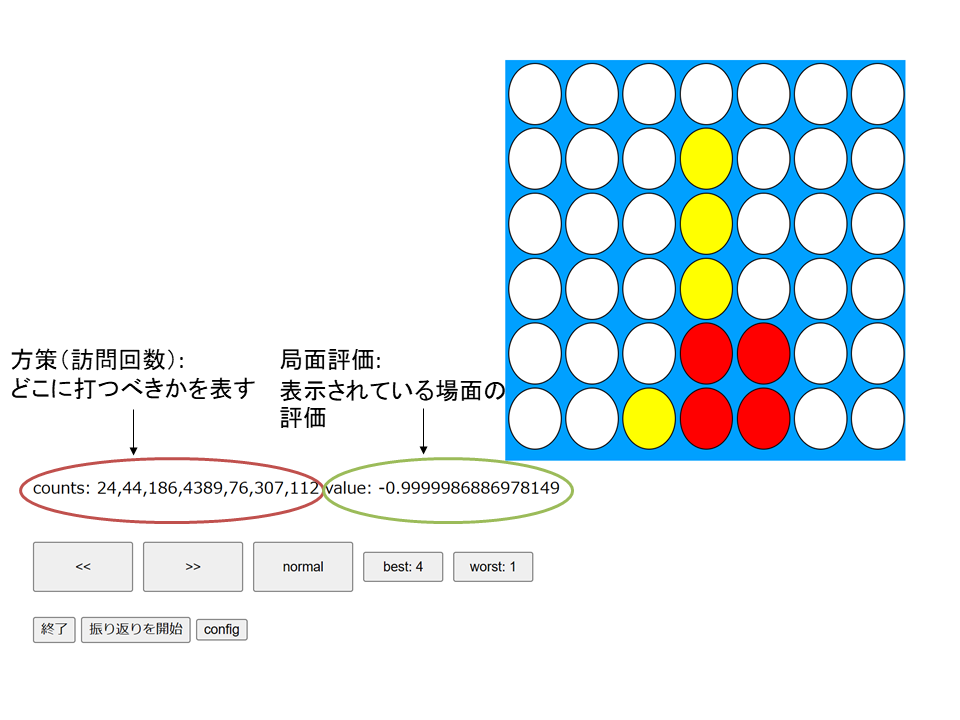
\includegraphics[width=\linewidth]{./figure/lookBack.png}}
	\caption{振り返り画面}
	\label{fig:lookBack}
\end{figure}
数字が描かれたボタンは列のインデックスを表しており,図\ref{fig:trajSystem}に示すように各ボタンを押した際にその列を選択した場合の想定図と局面評価を確認できる.
図\ref{fig:trajSystem}では「4」と描かれたボタンを押したため4列目を選択した場合の進行図が表示されている.
\begin{figure}[t]
    \centering
    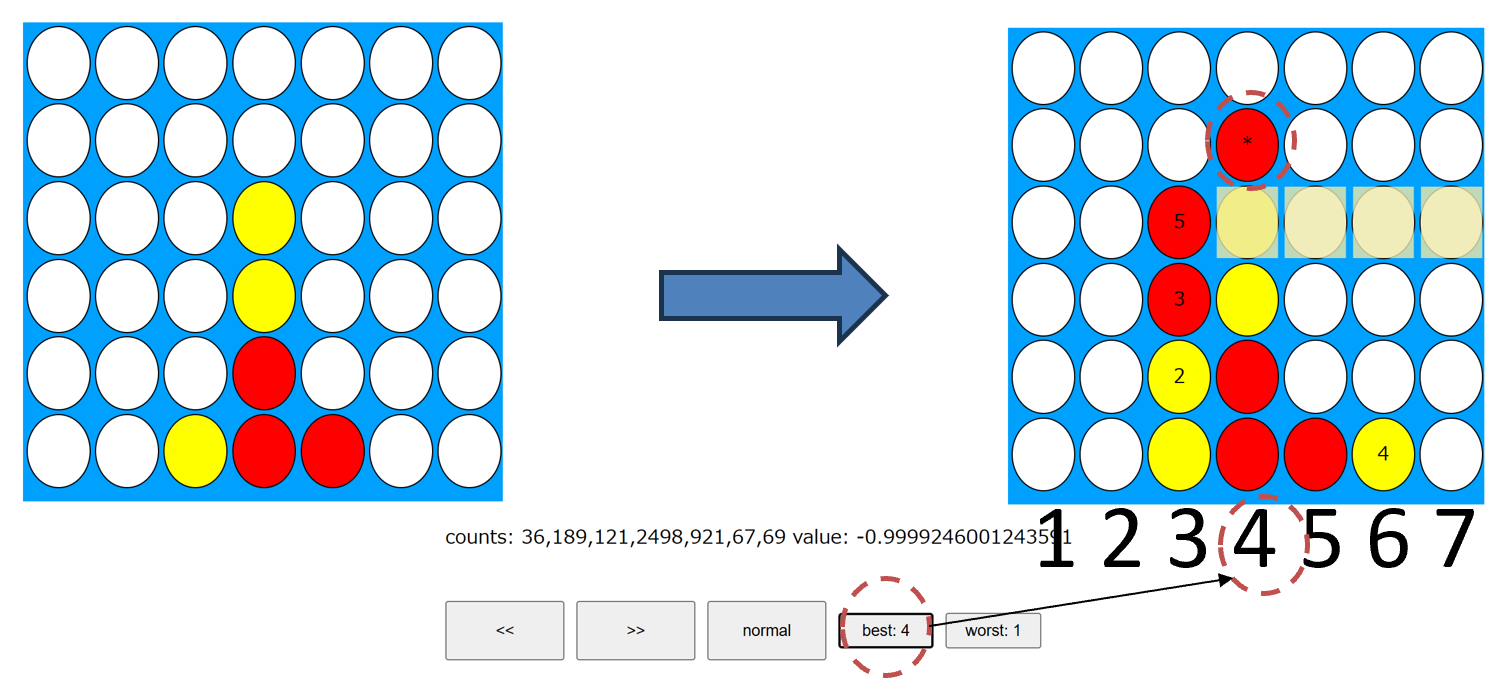
\includegraphics[width=\linewidth]{./figure/4-traj.png}
	\caption{進行図の表示}
	\label{fig:trajSystem}
\end{figure}
\subsection{インタフェース実験の評価指標}
インタフェース実験の評価指標は主観評価と客観評価の2つに分けられる.
主観評価は被験者による五段階評価であり,「タスクの熟達度に関連する質問」((a))と「タスクの楽しさや面白さに関連する質問」((b))の2つに分けられる.
具体的な質問事項は付録Dに記載する.
客観評価はグループA(提案手法)の被験者とグループB(比較手法)の被験者の対戦成績である.

\subsection{実験結果(インタフェース実験)}
進行図で提示される先読みの手数ごとに主観評価の平均値($1\sim5$)を表\ref{table:system-3}, 表\ref{table:system-5}, 表\ref{table:system-7}, 表\ref{table:system-100}に示す.
先読みの手数は${3, 5, 7, \textrm{制限なし}}$の4種類であり,先読みの手数ごとに図\ref{fig:see}に示すように提示される進行図中の手数が変化する.
先読みの手数に関わらず,AIが予測する進行において最終的に4つ以上の石が並ぶ座標は強調表示される.
\begin{figure}[t]
    \centering
    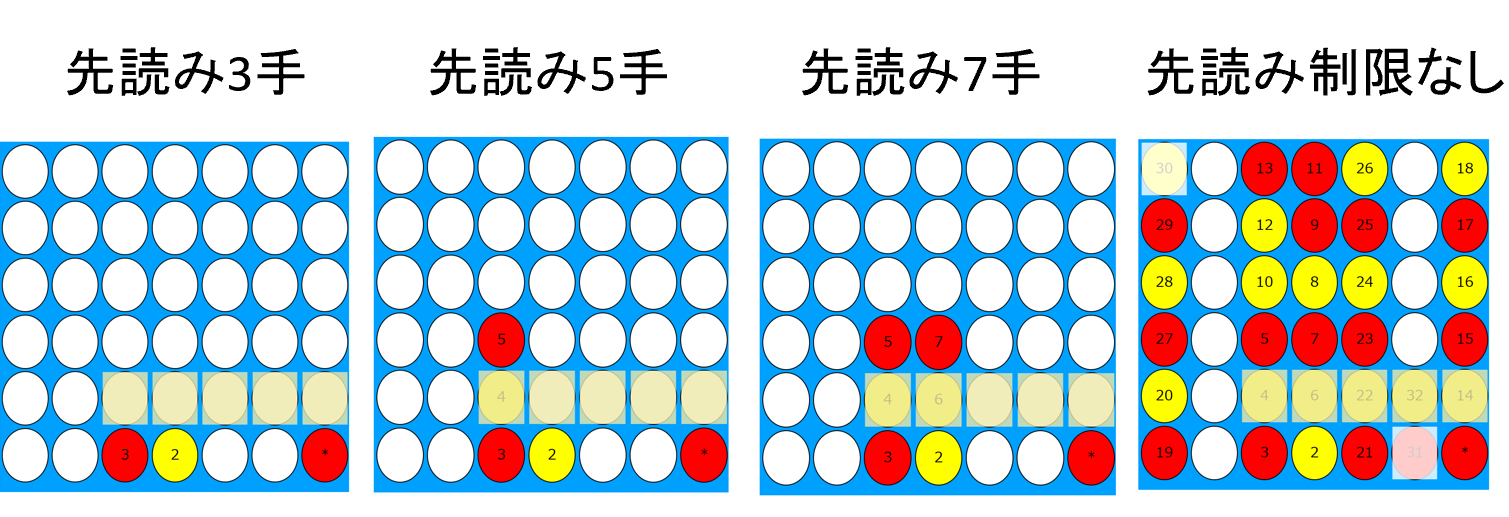
\includegraphics[width=\linewidth]{./figure/see.png}
	\caption{進行図の表示}
	\label{fig:see}
\end{figure}
先読み手数が3手または先読み手数制限なしの場合に,提案手法は比較手法に対して高い結果を示した.
表\ref{table:system-3}, 表\ref{table:system-5}, 表\ref{table:system-7}, 表\ref{table:system-100}に対して
t検定を行ったが,いずれも有意な差は見当たらなかった.
\begin{table}[H]
    \caption{先読み手数3手の場合(インタフェース実験)}
    \label{table:system-3}
    \scriptsize
    \centering
    \resizebox{\linewidth}{!}{
        \begin{tabular}{c|l||c|c}
            \multicolumn{2}{c}{質問} & \multicolumn{2}{c}{主観評価} \\ \hline \hline
            質問の種類 & 質問の内容& B(比較手法) & A(提案手法)  \\ \hline 
            (a) & 振り返りによって成長したと感じましたか & 3.17 & \bf{3.29} \\
            & 振り返りによってAIの意図を掴むことができたと感じますか & \bf{2.67} & 2.43 \\
            & (2回目のみ) 1回目に比べて成長したと感じますか& \bf{4.33} & 2.75  \\ \hline
            (b) & 今後も connect4 をプレイするときにこのシステムを使いたいと思いましたか & 3.67 & \bf{3.71} \\
            & システムにより振り返りが楽しくなったと感じますか& \bf{3.60} & {3.57}  \\
        \end{tabular}
    }
    
\end{table}
\begin{table}[H]
    \caption{先読み手数5手の場合(インタフェース実験)}
    \scriptsize
    \centering
    \resizebox{\linewidth}{!}{
        \begin{tabular}{c|l||c|c}
            \multicolumn{2}{c}{質問} & \multicolumn{2}{c}{主観評価} \\ \hline \hline
            質問の種類 & 質問の内容& B(比較手法) & A(提案手法)  \\ \hline 
            (a) & 振り返りによって成長したと感じましたか& \bf{4.00} & 3.00  \\
            & 振り返りによってAIの意図を掴むことができたと感じますか& \bf{4.00} & 2.60  \\
            & (2回目のみ) 1回目に比べて成長したと感じますか& \bf{4.33} & 3.67  \\ \hline
            (b) & 今後も connect4 をプレイするときにこのシステムを使いたいと思いましたか & \bf{4.80} & 4.00 \\
            & システムにより振り返りが楽しくなったと感じますか & \bf{4.60}  & 4.20\\
        \end{tabular}
    }
    \label{table:system-5}
\end{table}
\begin{table}[H]
    \caption{先読み手数7手の場合(インタフェース実験)}
    \scriptsize
    \centering
    \resizebox{\linewidth}{!}{
        \begin{tabular}{c|l||c|c}
            \multicolumn{2}{c}{質問} & \multicolumn{2}{c}{主観評価} \\ \hline \hline
            質問の種類 & 質問の内容 & B(比較手法) & A(提案手法)\\ \hline 
            (a) & 振り返りによって成長したと感じましたか& \bf{4.33} & {3.83}  \\
            & 振り返りによってAIの意図を掴むことができたと感じますか & \bf{3.67} & 2.67 \\
            & (2回目のみ) 1回目に比べて成長したと感じますか & \bf{4.33} & 2.75 \\ \hline
            (b) & 今後も connect4 をプレイするときにこのシステムを使いたいと思いましたか& \bf{4.67} & 4.17  \\
            & システムにより振り返りが楽しくなったと感じますか & \bf{3.50} & 3.00 \\
        \end{tabular}
    }
    \label{table:system-7}
\end{table}
\begin{table}[H]
    \caption{先読み手数制限なしの場合(インタフェース実験)}
    \scriptsize
    \centering
    \resizebox{\linewidth}{!}{
        \begin{tabular}{c|l||c|c}
            \multicolumn{2}{c}{質問} & \multicolumn{2}{c}{主観評価} \\ \hline \hline
            質問の種類 & 質問の内容 & B(比較手法) & A(提案手法) \\ \hline 
            (a) & 振り返りによって成長したと感じましたか & 4.00 & \bf{4.25} \\
            & 振り返りによってAIの意図を掴むことができたと感じますか& 3.00  & \bf{3.50} \\
            & (2回目のみ) 1回目に比べて成長したと感じますか& \bf{4.33}  & 2.75 \\ \hline
            (b) & 今後も connect4 をプレイするときにこのシステムを使いたいと思いましたか& 4.00  & \bf{4.5} \\
            & システムにより振り返りが楽しくなったと感じますか & 4.40  & \bf{4.75}\\
        \end{tabular}
    }
    \label{table:system-100}
\end{table}
また,第2段階である被験者同士の対戦結果を表\ref{table:result-battle}に示す.
付録Dに示すように被験者1人に対して2回対戦を行った.結果として示すscoreは勝利を1,敗北を-1,引き分けを0
とした2回の対戦の平均値として定義される.
提案手法を用いて訓練を行ったグループ(A)は比較手法を用いて訓練を行ったグループ(B)よりも高い
勝率を記録し,scoreはマン・ホイットニーのU検定において有意な差を示した.
\begin{table}[H]
	\caption{対戦の結果(インタフェース実験)}
    \label{table:result-battle}
	\centering
	\scalebox{0.98}[0.98]{
		\begin{tabular}{c|c|c}
            グループ & B(比較手法)  & A(提案手法) \\ \hline
			mean score &  -0.15*   & \bf{0.25*}\\ \hline
		\end{tabular}
	}
	
\end{table}
また,第3章で示した新たな重要度の定義(式\ref{new-imp})の妥当性を検証するため,盤面$s$の重要度$I(s)$と被験者が$s$の進行図を
見た時間$t$の相関を調査した.比較手法には式\ref{imp}の定義を用いた.
表\ref{table:result-imp}に示したように,いずれの手法による重要度も$t$との有意な相関が見られなかった.
\begin{table}[H]
	\caption{手法別の重要度と$t$の相関(インタフェース実験)}
    \label{table:result-imp}
	\centering
	\scalebox{0.98}[0.98]{
		\begin{tabular}{c|c|c}
			日数& 比較手法& 提案手法  \\ \hline
			1日目& \bf{-0.034}& {-0.035}\\
            2日目& \bf{0.067}& {-0.083}\\
		\end{tabular}
	}
	
\end{table}


\subsection{考察(インタフェース実験)}


提案手法を用いたグループAがグループBを上回る評価を得たのは,主に先読みが最も短い3手の場合と最も長い制限なしの場合となった.

先読み3手,制限なしの場合のデータをさらに1日目,2日目で分類した結果,
\begin{itemize}
    \item 先読み3手の場合は1日目
    \item 先読み制限なしの場合は2日目
\end{itemize}

の方がよりグループAからの評価が高いことが分かった.
付録\ref{chap:system}で述べるように,1日目と2日目ではGUIの設定に差があり
1日目のGUIでは全ての選択肢(最大7種)を起点とした進行図を閲覧可能であるのに対し,2日目のGUIでは起点となる選択肢を
2つに制限した.
そのため,2日目は被験者が見られる進行図の数が1日目の約$\frac{1}{3}$となる.

そのため,「1日目に先読み3手の場合」と「2日目に先読み制限なし」の場合に被験者が受け取る情報量は近しいと推測される.

また,データを「被験者のグループ,日にち,先読み手数」によって分類し,「振り返りによってAIの意図を掴むことができたと感じますか」という質問に対する評価(以下把握満足度と表記)の降順に
並べ直した結果を表\ref{table:order}に示す.
\begin{table}[H]
	\caption{把握満足度(インタフェース実験)}
    \label{table:order}
    \scriptsize
	\centering
	\scalebox{0.98}[0.98]{
		\begin{tabular}{c|c|c||c}
			グループ& 日 & 先読み手数 &把握満足度 \\ \hline
			B & 2 & 5 & 4.67\\
            B & 2 & 7 & 4.00\\
            A & 1 & 制限なし& 3.50\\
            A & 2 & 制限なし& 3.50\\
            B & 1 & 3& 3.50\\
            B & 1 & 制限なし& 3.33\\
            A & 1 & 3& 3.33\\
            \multicolumn{4}{c}{(\ldots)}\\
            A & 2 & 3 & 1.75\\
            B & 1 & 3 & 1.50\\

		\end{tabular}
	}
	
\end{table}

グループAのデータを日にちと先読み手数で分けた場合最も把握満足度が高いのは
「2日目に先読み制限なし」,次いで「1日目に先読み制限なし」,「1日目に先読み3手」となった.
最も情報が少ない「2日目に3手」はグループAの全8パターン中最下位となった.\\


グループBに対しても同様に「振り返りによってAIの意図を掴むことができたと感じますか」への評価を集計した結果,
最も評価が高いのは「2日目に5手」,次いで「2日目に7手」,「1日目に3手」となった.\\



また,付録\ref{chap:data}の表\ref{table:tail}より提案手法が示す1組の状態$s$,行動$a$について示す軌跡の数$n$の平均は約10であるため,比較手法が示す情報量は提案手法の約$\frac{1}{10}$となる.
また,先読みの手数に制限が無い場合の手数の平均は約15手である.
そのため提示する情報量が大きい程評価が高くなるわけではなく,手法ごとに被験者が適切と感じる情報量が存在すると推測される.\\

以上の考察
を踏まえて,被験者に対して提示する情報を最小化した上で適切な情報量を調査するため,
先読みを1$\sim$5手として再実験を行った.
インタフェース実験では補助として提示した訪問回数,局面評価に注目する被験者が多く見られたため,訪問回数「count」(訪問回数)の表示を廃止し,「value」(局面評価)と進行図の閲覧は被験者の手番(先番)となる盤面でのみ可能とした.

結果を\ref{fig:add-result}に示す.

\begin{table}[H]
    \caption{先読み手数制限なしの場合(追加実験)}
    \scriptsize
    \centering
    \resizebox{\linewidth}{!}{
        \begin{tabular}{c|l||c|c}
            \multicolumn{2}{c}{質問} & \multicolumn{2}{c}{主観評価} \\ \hline \hline
            質問の種類 & 質問の内容& B & A  \\ \hline 
            (a) & 振り返りによって成長したと感じましたか& \bf{3.80} & 3.00  \\
            & 振り返りによってAIの意図を掴むことができたと感じますか& 2.80 & \bf{3.00} \\
            & 振り返りでは対戦を振り返るのに十分な量の情報を受け取ることができたと思いますか& 3.00 & \bf{3.60}  \\ \hline
            (b) & 今後も connect4 をプレイするときにこのシステムを使いたいと思いましたか& 3.80 & \bf{4.2}  \\
            & システムにより振り返りが楽しくなったと感じますか& \bf{4.20} & 3.6  \\
        \end{tabular}
    }
    \label{table:add-result}
\end{table}


把握満足度と「充分な情報量」の平均は提案手法の方が高くなった.そのため,被験者が比較手法では情報量が不十分であると感じている
際に,提案手法で情報を補足することには一定の意義があると推測される.ただし,t検定による有意差は見当たらなかった.
また,先読みが1手や2手の場合は,提案手法による軌跡が枝分かれせず,結果的に表示される軌跡の数が小さくなる.
そのため,提案手法と比較手法の差異は「決定木中のどの部分を取り出すか」の差異となる.
付録\ref{chap:alg}の\ref{sec:fix}で述べたように提案手法で示す進行図は盤面の局面評価と符合するように調整されていることも評価に寄与したと
考えられる.